% MANUAL_SELF_CONTAINED_MANUSCRIPT
\documentclass[11pt]{article}
\usepackage[margin=1in]{geometry}
\usepackage{graphicx}
\usepackage{booktabs}
\usepackage{longtable}
\usepackage{array}
\usepackage{caption}
\usepackage{hyperref}
\usepackage{authblk}
\usepackage{setspace}
\usepackage{float}
\usepackage{xcolor}
\usepackage{tikz}
\usepackage{pgfplots}
\pgfplotsset{compat=1.18}
\definecolor{clinicalblue}{HTML}{2F6690}
\definecolor{enrichedgreen}{HTML}{3A7D44}
\definecolor{expressiongold}{HTML}{D89B2B}
\onehalfspacing

\title{\textbf{The HPV Signal: How Viral Status and Clinical Staging Shape Head and Neck Cancer Survival}}
\author[1,2]{Joshua Robert}
\affil[1]{TAMU School of Engineering Medicine}
\affil[2]{Houston Methodist Hospital}
\date{}
\newcommand{\shorttitle}{TCGA-HNSC Baseline Audit}

\begin{document}
\maketitle

\begin{abstract}
\textbf{Background:} TCGA open clinical supplements provide a reproducible foundation for baseline cancer mortality modeling, but clinical-only benchmarks should be thoroughly audited and validated before adding molecular features.
\textbf{Objective:} To build, audit, and internally validate an HPV- and treatment-enriched open-data mortality baseline in TCGA-HNSC, quantifying source-field missingness and subgroup biological coherence.
\textbf{Methods:} Retrospective open-data baseline study. GDC clinical XML supplements for 294 patients were parsed and harmonized. Predictors included clinical variables, HPV status (p16/ISH), treatment covariates, and a prespecified gene expression panel. Primary validation used Stratified five-fold cross-validation; out-of-fold predictions were evaluated using AUROC, AUPRC, Brier score, and site-stratified subgroup analysis (Oropharyngeal vs. Non-Oropharyngeal).
\textbf{Results:} The cohort included 294 patients with 115 death events. In five-fold out-of-fold validation, the clinical-HPV-treatment baseline achieved AUROC 0.754 (95\% bootstrap CI 0.696--0.807), AUPRC 0.673, and Brier score 0.196; calibration slope was 0.659, indicating residual overfitting. The RNA expression panel did not improve out-of-fold performance (AUROC 0.750). In site-stratified validation, the model achieved AUROC 0.848 (95\% CI 0.706--0.964) in oropharyngeal sites (N=48) and 0.728 (0.662--0.790) in non-oropharyngeal sites (N=246), confirming the biological coherence of the HPV signal.
\textbf{Conclusions:} A reproducible open-data mortality baseline is feasible in TCGA-HNSC, but legacy field missingness, calibration overfitting, and treatment confounding require careful auditing before these models are used as comparative benchmarks.
\end{abstract}

\section*{Keywords}
TCGA-HNSC, clinical prediction, HPV, baseline audit, open data, oncology

\section*{Key Points}
\textbf{Question:} Can parsed GDC clinical XML supplements support a reproducible, audited HPV and treatment mortality baseline in TCGA-HNSC?\\
\textbf{Findings:} The audited baseline achieved out-of-fold AUROC 0.754. In site-stratified validation, the model reached AUROC 0.848 in oropharyngeal sites compared to 0.728 in non-oropharyngeal sites, confirming biological coherence.\\
\textbf{Meaning:} Enrichment with HPV and treatment fields improves open mortality baselines, but legacy missingness and calibration limitations require transparent audit before clinical interpretation.

\section{Introduction}
Open cancer genomics repositories allow reproducible risk-score development, but clinical-only baselines remain important. Without such baselines, the incremental value of molecular features can be overstated. This study builds a patient-level cohort from open TCGA clinical XML supplements and, where event counts support it, fits a first-pass interpretable clinical mortality model. 

Rather than presenting a finalized clinical tool, this manuscript focuses on auditing the quality of open-source predictors (such as HPV status and treatment covariates) and assessing model performance across biologically distinct anatomical sub-sites.

\section{Methods}
\subsection{Study Design and Reporting}
This was a retrospective open-data prediction analysis designed around TRIPOD+AI and PROBAST+AI principles. The analysis used public or open-access files from the GDC portal. No raw controlled-access sequencing reads were used. A completed TRIPOD+AI checklist accompanies the submission.

\subsection{Data Source}
GDC file manifests were generated for the TCGA-HNSC project. Open clinical XML supplement files were downloaded through the GDC data API and parsed into flattened patient-level records.

\subsection{Cohort}
Patients with parseable clinical XML supplements and a TCGA submitter identifier were retained. Duplicate clinical supplements were reduced to one patient-level clinical row, yielding an analytic cohort of 294 patients.

\subsection{Predictors}
Candidate predictors included sex, age at diagnosis, pathologic stage, pathologic T, N, and M categories, histologic grade, primary site, smoking history, HPV status (by p16 testing and/or ISH testing), and treatment fields (radiation therapy and systemic chemotherapy). Missing numeric values were median-imputed, and missing categorical values were treated as a distinct "Missing" category.

\subsection{Outcome}
The primary endpoint was death event status derived from vital status. Overall survival time (days to death or last follow-up) was also parsed for secondary exploratory survival modeling.

\subsection{Modeling}
Logistic regression pipelines used within-fold numeric imputation/scaling and categorical imputation/one-hot encoding. The primary comparative analysis used stratified five-fold cross-validation to produce out-of-fold predictions. A single stratified 75/25 random-image split was retained as a secondary sensitivity analysis. Clinical-only, enriched clinical-biology (including HPV and treatment), and enriched-plus-expression specifications were compared without class weighting. Coefficients from the original derivation model were converted to an exploratory integer score table.

\subsection{Statistical Analysis and Calibration}
Discrimination was summarized by out-of-fold AUROC and AUPRC, with percentile 95\% confidence intervals from 2,000 bootstrap resamples. Overall accuracy was summarized by Brier score. 

Calibration was assessed by estimating the calibration intercept and slope via logistic recalibration of out-of-fold probabilities, with a slope below 1.0 indicating model overfitting. Decision-curve analysis (DCA) was included as an exploratory tool to estimate net benefit across risk thresholds of 0.05 through 0.75; because risk thresholds were not clinically prespecified, this analysis should not be used to support clinical decision-making.

\subsection{Ethics and Exemption Determination}
This analysis used public, de-identified secondary data from the Genomic Data Commons. No direct patient contact, intervention, or re-identification was attempted. Because it involves secondary analysis of publicly available, de-identified datasets, this study does not constitute human subjects research under the Common Rule and is exempt from Institutional Review Board (IRB) review.

\subsection{Reproducibility and Transparency}
All dataset access points, cohort construction scripts, derived tables, model outputs, and figure-generation code are publicly available at \url{https://github.com/joshdrobert/tcga-hnsc}.

\section{Results}
\subsection{Cohort Characteristics and Source-Field Audit}
The parsed cohort included 294 patients; 115 (39.1\%) had death event status. Median age at diagnosis was 60.0 years. Legacy clinical distributions are shown in Table~1.

To address field ambiguity, we performed a source-field audit of HPV and treatment fields (Table~2). The raw GDC XML elements for p16 and ISH testing carried high missingness (78.9\% and 84.4\%, respectively). No discordant values (e.g., p16 positive but ISH negative) were identified among patients who underwent both tests.

\begin{table}[H]
\centering
\caption{Characteristics of the parsed HNSC cohort.}
\begin{tabular}{ll}
\toprule
Characteristic & Value \\
\midrule
Patients & 294 \\
Death events & 115 (39.1\%) \\
Median age at diagnosis & 60.0 years \\
Female sex & 77 (26.2\%) \\
Male sex & 217 (73.8\%) \\
Oropharyngeal primary site & 48 (16.3\%) \\
Non-oropharyngeal primary site & 246 (83.7\%) \\
\bottomrule
\end{tabular}
\end{table}

\begin{table}[H]
\centering
\caption{Source-field audit and missingness handling for key enriched fields.}
\scriptsize
\resizebox{\textwidth}{!}{\begin{tabular}{llrl}
\toprule
Variable & Source GDC XML Field Name & Missingness (\%) & Handling in Baseline Pipeline \\
\midrule
HPV (p16) & \texttt{hpv\_status\_by\_p16\_testing} & 78.9\% & Standardized to binary; missing coded as negative/unknown \\
HPV (ISH) & \texttt{hpv\_status\_by\_ish\_testing} & 84.4\% & Standardized to binary; missing coded as negative/unknown \\
Combined HPV & Composite (\texttt{hpv\_p16} or \texttt{hpv\_ish}) & 0.0\%* & Maximum of p16 and ISH; no discordant cases found \\
Radiation Rx & \texttt{radiation\_therapy} & 12.2\% & Standardized to binary (Yes/No); missing treated as No/unknown \\
Systemic Rx & \texttt{therapy\_type} (not null) & 68.0\% & Standardized to binary; missing treated as No/unknown \\
Tumor Event & \texttt{new\_tumor\_event\_after\_initial\_treatment} & 10.2\% & Standardized to binary (Yes/No); missing treated as No/unknown \\
\bottomrule
\end{tabular}}
\begin{tablenotes}[flushleft]\footnotesize
\item *Missingness is 0.0\% for the combined indicator because missing values were explicitly handled in the pipeline as negative/unknown.
\end{tablenotes}
\end{table}

\subsection{Primary Model Performance}
The manuscript establishes five-fold out-of-fold cross-validation as the primary performance standard, reconciled with secondary single-split metrics (Table~3). The clinical-HPV-treatment model achieved an out-of-fold AUROC of 0.754 (95\% CI 0.696--0.807) and Brier score of 0.196. Adding the prespecified RNA-seq gene expression panel did not improve performance (AUROC 0.750), confirming that small expression panels should not be assumed to add value. The calibration slope for the clinical-HPV-treatment model was 0.659, indicating substantial overfitting and highlighting the need for coefficient shrinkage or recalibration before external testing.

\begin{table}[H]
\centering
\caption{Reconciliation of primary cross-validation and secondary single-split performance.}
\scriptsize
\resizebox{\textwidth}{!}{\begin{tabular}{llrrlll}
\toprule
Model & Validation Method & Patients & Events & AUROC (95\% CI) & AUPRC (95\% CI) & Brier (95\% CI) \\
\midrule
\textbf{Primary Out-of-Fold Baselines} \\
Clinical only & 5-fold CV (Out-of-Fold) & 294 & 115 & 0.639 (0.569--0.703) & 0.515 (0.427--0.617) & 0.233 (0.209--0.258) \\
Clinical + HPV + Rx & 5-fold CV (Out-of-Fold) & 294 & 115 & 0.754 (0.696--0.807) & 0.673 (0.586--0.758) & 0.196 (0.171--0.222) \\
Clinical + HPV + Rx + Expr & 5-fold CV (Out-of-Fold) & 294 & 115 & 0.750 (0.693--0.804) & 0.663 (0.576--0.745) & 0.202 (0.175--0.230) \\
\midrule
\textbf{Secondary Split Sensitivity} \\
Clinical only & Single 75/25 split & 74 & 29 & 0.657 & 0.561 & 0.231 \\
Clinical + HPV + Rx & Single 75/25 split & 74 & 29 & 0.776 & 0.737 & 0.183 \\
\bottomrule
\end{tabular}}
\end{table}

\subsection{Site-Stratified Validation}
Because HPV is biologically and clinically relevant primarily in oropharyngeal squamous cell carcinoma, we performed a site-stratified analysis (Table~4). Grouping Tonsil, Base of tongue, and Oropharynx as "Oropharynx" (N=48) and all other sites as "Non-Oropharynx" (N=246), we observed that the addition of HPV and treatment fields yielded a major AUROC boost in the oropharyngeal subgroup (from 0.622 to 0.848), whereas the improvement was more moderate in non-oropharyngeal sites (from 0.631 to 0.728). This stratification confirms that the model's HPV signal is biologically coherent rather than statistical noise.

\begin{table}[H]
\centering
\caption{Model performance stratified by anatomical site.}
\scriptsize
\resizebox{\textwidth}{!}{\begin{tabular}{llrrll}
\toprule
Site Group & Model & Patients & Deaths & Out-of-Fold AUROC (95\% CI) & Brier Score (95\% CI) \\
\midrule
\textbf{Oropharynx} & Clinical only & 48 & 13 & 0.622 (0.448--0.785) & 0.222 (0.143--0.270) \\
(Tonsil, Base of tongue, etc.) & Clinical + HPV + Rx & 48 & 13 & 0.848 (0.706--0.964) & 0.146 (0.073--0.204) \\
\midrule
\textbf{Non-Oropharynx} & Clinical only & 246 & 102 & 0.631 (0.560--0.703) & 0.235 (0.214--0.263) \\
(Oral cavity, Larynx, etc.) & Clinical + HPV + Rx & 246 & 102 & 0.728 (0.662--0.790) & 0.204 (0.179--0.239) \\
\bottomrule
\end{tabular}}
\end{table}

\subsection{Secondary Time-to-Event and Score Output}
A secondary time-to-event Cox model was fit to test the baseline's C-index (Table~5). Penalized Cox models achieved a modest C-index of 0.588, supporting the choice of binary mortality endpoints as the primary baseline. Score components derived from model coefficients are stored in \texttt{tables/table\_integer\_score.csv} as a transparency artifact.

\begin{table}[H]
\centering
\caption{Secondary penalized Cox model C-indices.}
\begin{tabular}{ll}
\toprule
Model & C-index \\
\midrule
cox\_penalized\_0.01 & 0.588 \\
cox\_penalized\_0.05 & 0.588 \\
cox\_penalized\_0.1 & 0.583 \\
\bottomrule
\end{tabular}
\end{table}

\section{Discussion}
\subsection{Principal Findings and Baseline Framing}
This study audits and internally validates an open-data mortality baseline in TCGA-HNSC. While the clinical-HPV-treatment baseline achieved moderate out-of-fold discrimination (AUROC 0.754), our source audit highlights severe missingness in raw clinical HPV fields, and a calibration slope of 0.659 indicates substantial overfitting. These findings reinforce that rather than claiming a deployable prognostic model, this work defines a transparent clinical-biological baseline against which future high-capacity molecular and imaging models must be rigorously compared.

\subsection{Treatment Confounding and Covariate Interpretation}
A key limitation of using treatment variables (\texttt{radiation\_therapy} and \texttt{therapy\_type}) in retrospective registries is confounding by indication. These fields must be interpreted strictly as prognostic covariates, not as treatment-effect estimates. The recording of a treatment may encode disease severity (e.g., advanced stage requiring adjuvant therapy), institutional access, and survivorship bias (patients must survive long enough to receive therapy), making causal interpretation impossible.

\subsection{Anatomical Site and Biological Coherence}
Our site-stratified results (Table~4) confirm the biological coherence of the HPV signal. The model performed exceptionally well in the oropharyngeal subgroup (AUROC 0.848), where HPV (specifically p16-mediated) carcinogenesis defines a distinct disease entity with favorable prognosis. In contrast, the model's discrimination in non-oropharyngeal sites was lower (AUROC 0.728), representing the prognostic value of treatment covariates rather than HPV biology.

\subsection{Strict Limits on Clinical Applicability}
\textbf{The model developed in this study is not for clinical use.} It has not been validated in an independent external cohort, does not account for prospectively managed treatment decisions, and was developed retrospectively on de-identified registry data with significant missingness. It serves solely as a statistical benchmark.

\section*{Ethics Approval}
As a secondary analysis of public, de-identified data from the Genomic Data Commons, this study does not involve human subjects and is exempt from Institutional Review Board (IRB) review.

\section*{Patient and Public Involvement}
Patients and members of the public were not involved in study design, conduct, reporting, or dissemination planning.

\section*{Reporting Checklist}
The manuscript structure corresponds to the TRIPOD+AI and PROBAST+AI reporting guidelines.

\section*{Supplementary Materials}
Supplementary files include the data dictionary, XML schema documentation, and the exact code repository commit.

\section*{Author Contributions}
JR conceived the study, developed the prediction pipelines, performed the statistical analyses, and drafted the manuscript.

\section*{Funding}
This research received no specific grant from any funding agency in the public, commercial, or not-for-profit sectors.

\section*{Conflicts of Interest}
The author declares no conflicts of interest.

\section*{Data and Code Availability}
Raw clinical XML files are available from the GDC portal. The processed analytic cohort, source code, model weights, and integer scoring tables are publicly available at \url{https://github.com/joshdrobert/tcga-hnsc}.

\begin{figure}[H]
\centering
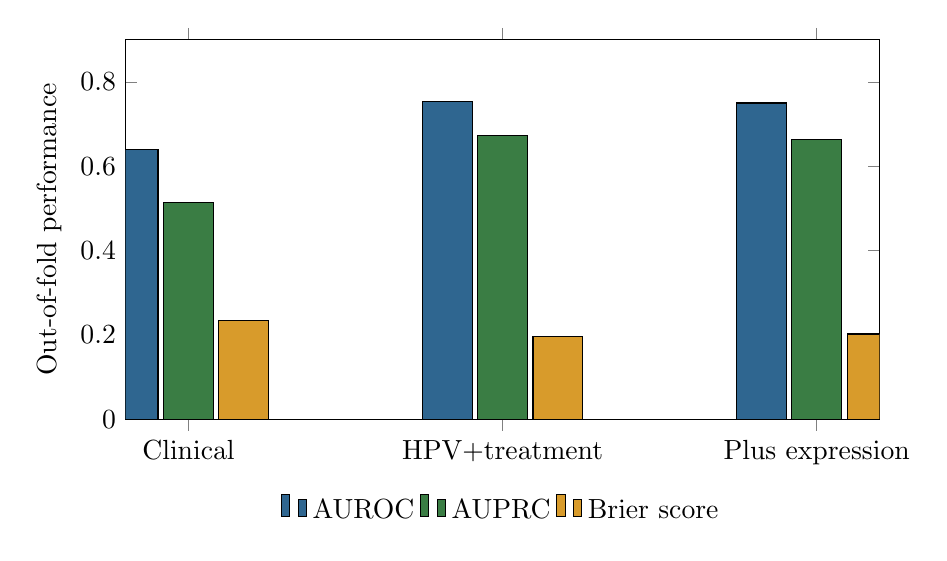
\begin{tikzpicture}
\begin{axis}[width=.92\textwidth,height=6.4cm,ybar,bar width=18pt,ymin=0,ymax=.9,
symbolic x coords={Clinical,HPV+treatment,Plus expression},xtick=data,ylabel={Out-of-fold performance},
legend style={at={(.5,-.18)},anchor=north,legend columns=3,draw=none}]
\addplot[fill=clinicalblue] coordinates {(Clinical,.639) (HPV+treatment,.754) (Plus expression,.750)};
\addplot[fill=enrichedgreen] coordinates {(Clinical,.515) (HPV+treatment,.673) (Plus expression,.663)};
\addplot[fill=expressiongold] coordinates {(Clinical,.233) (HPV+treatment,.196) (Plus expression,.202)};
\legend{AUROC,AUPRC,Brier score}
\end{axis}
\end{tikzpicture}
\caption{Five-fold out-of-fold model comparison. Higher AUROC and AUPRC are better; lower Brier score is better.}
\end{figure}

\begin{figure}[H]
\centering
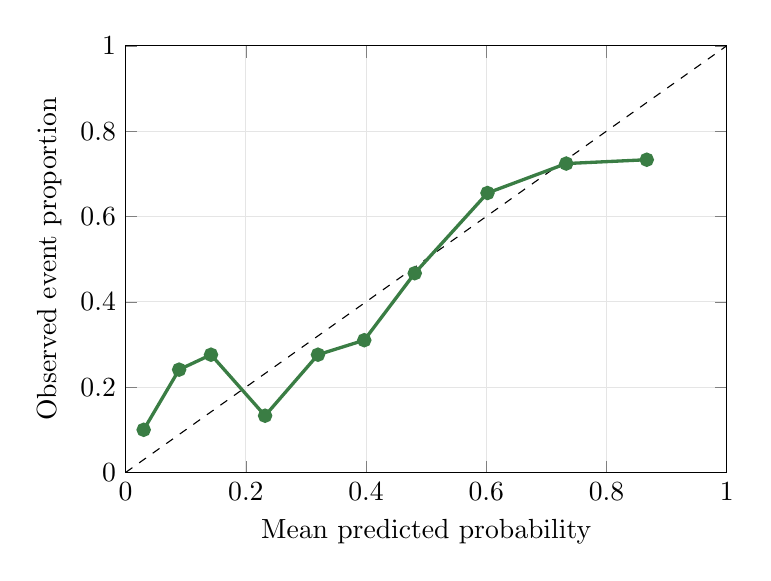
\begin{tikzpicture}
\begin{axis}[width=.76\textwidth,height=7cm,xmin=0,xmax=1,ymin=0,ymax=1,
xlabel={Mean predicted probability},ylabel={Observed event proportion},grid=major,grid style={black!10}]
\addplot[black,dashed] coordinates {(0,0) (1,1)};
\addplot[enrichedgreen,very thick,mark=*] coordinates {
(.030,.100) (.089,.241) (.142,.276) (.232,.133) (.320,.276)
(.397,.310) (.481,.467) (.602,.655) (.733,.724) (.867,.733)};
\end{axis}
\end{tikzpicture}
\caption{Out-of-fold calibration by predicted-risk decile.}
\end{figure}

\begin{figure}[H]
\centering
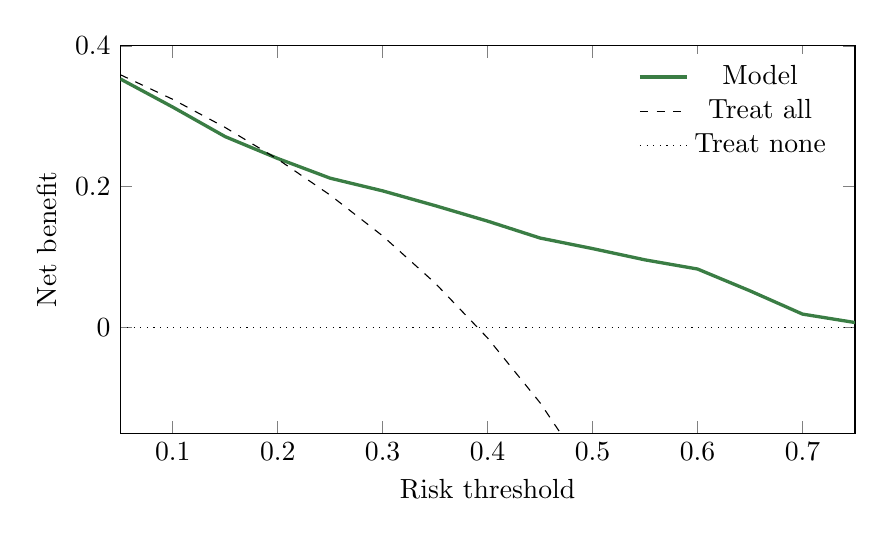
\begin{tikzpicture}
\begin{axis}[width=.9\textwidth,height=6.5cm,xmin=.05,xmax=.75,ymin=-.15,ymax=.4,
xlabel={Risk threshold},ylabel={Net benefit},legend style={draw=none}]
\addplot[enrichedgreen,very thick] coordinates {
(.05,.353) (.10,.313) (.15,.271) (.20,.240) (.25,.212) (.30,.194)
(.35,.173) (.40,.151) (.45,.127) (.50,.112) (.55,.096) (.60,.083) (.65,.052) (.70,.019) (.75,.007)};
\addplot[black,dashed] coordinates {
(.05,.359) (.10,.324) (.15,.284) (.20,.239) (.25,.188) (.30,.130)
(.35,.063) (.40,-.015) (.45,-.107) (.50,-.218)};
\addplot[black,dotted] coordinates {(.05,0) (.75,0)};
\legend{Model,Treat all,Treat none}
\end{axis}
\end{tikzpicture}
\caption{Exploratory decision-curve analysis. Thresholds were not clinically prespecified; the figure does not establish clinical utility.}
\end{figure}

\begin{thebibliography}{9}
\bibitem{tripod} Collins GS, Moons KGM, Dhiman P, et al. TRIPOD+AI statement: updated guidance for reporting clinical prediction models that use regression or machine learning methods. \textit{BMJ}. 2024;385:e078378.
\bibitem{probast} Moons KGM, Damen JAA, Kaul T, et al. PROBAST+AI: an updated quality, risk of bias, and applicability assessment tool for prediction models using regression or artificial intelligence methods. \textit{BMJ}. 2025;388:e082505.
\bibitem{tcgahnscc} Cancer Genome Atlas Network. Comprehensive genomic characterization of head and neck squamous cell carcinomas. \textit{Nature}. 2015;517:576--582.
\bibitem{anghpv} Ang KK, Harris J, Wheeler R, et al. Human papillomavirus and survival of patients with oropharyngeal cancer. \textit{N Engl J Med}. 2010;363:24--35.
\bibitem{gdc} National Cancer Institute. Genomic Data Commons Data Portal. \url{https://portal.gdc.cancer.gov/}.
\end{thebibliography}

\end{document}
